\documentclass[14pt]{article}
\usepackage{styles}
\usepackage{graphicx}


\begin{document}

    \titlewithlabnum

    \tableofcontents
    \newpage


    \section{Завдання:}
    Розробити програму для побудови графіків довільних функцій y = f(x)


    \section{Обгрунтування проектного рішення}
    Проектне рішення для створення програми для побудови графіків довільних функцій Ethereal Plot було прийняте на основі важливих факторів:

    \begin{enumerate}
        \item Простота \\
        Проект "Ethereal Plot" було розроблено для створення високоефективного та інтуїтивно зрозумілого інструменту для побудови графіків довільних функцій на платформі Android з використанням Jetpack Compose.
        \item Функціональність
        \begin{enumerate}
            \item  Масштабування та Зсув \\
            Зручний інтерфейс для зміни масштабу графіків та їх зсув для детальнішого вивчення областей інтересу.
            \item Колірна Кодифікація \\
            Різні функції мають різний колір для зручності візуального розрізнення на графіку.
            \item  Збереження та Обмін \\
            Можливість зберігання графіків для майбутнього використання.
        \end{enumerate}
    \end{enumerate}
    
    \section{Аналіз можливих варіантів рішення для проекту}

        \subsection{Графічний Двигун:}
           - \textit{OpenGL ES:} Використання графічного двигуна, такого як OpenGL ES, може забезпечити високу ефективність у побудові графіків та взаємодії з ними. Однак це може призвести до складнішого коду та вищого рівня абстракції.
        
        \subsection{Альтернативні бібліотеки для побудови графіків:}
           - \textit{MPAndroidChart:} Використання сторонньої бібліотеки, такої як MPAndroidChart, може надати широкий функціонал для побудови графіків з мінімальними зусиллями.
        
        \subsection{Мова програмування:}
           - \textit{Kotlin:} Kotlin є офіційною мовою для розробки Android, і використання її підвищує читабельність коду та гарантує високий рівень безпеки.
        
        \subsection{Моделювання даних:}
           - \textit{Flow та LiveData:} Використання Flow та LiveData для реактивного програмування може спростити оновлення графіків під час зміни даних.
        
        \subsection{5. Збереження та обмін даними:}
           - \textit{SQLite або Room:} Використання вбудованих інструментів для роботи з базами даних сприяє зручному збереженню та обміну збереженими графіками.
        
        \subsection{Тестування:}
           - \textit{JUnit та Espresso:} Використання JUnit для юніт-тестування та Espresso для інтеграційного тестування допомагає забезпечити стабільність та коректність функціоналу.
        
        \subsection*{UI та UX:}
           - \textit{Material Design:} Використання принципів Material Design дозволяє створити сучасний та інтуїтивно зрозумілий інтерфейс для користувачів.
        
        \subsection*{Документація та Підтримка:}
           - \textit{Dokka:} Використання Dokka для генерації документації сприяє кращому розумінню коду та полегшує процес розробки.
        


    \section{Пояснювальна записка}
    Програма Ethereal Plot, андроїд дотаток для побудови графіків.


    \subsection{Основні функції}
    Додаток може малювати різноманітні функції, окрім тих, що мають вертикальні асимптоти. \\
    Додаток має можливість зміни кольору, відключення та видалення функцій. \\
    Додаток підтримує material ui 3, і є зручним та інтуїтивним

    
    \section{Теоретичні положення}
    \subsection{Jetpack Compose}
    \href{https://developer.android.com/jetpack/compose/documentation}{Посилання на документацію, в якій описані всі положення}

    \subsection{Мова Програмування Kotlin}
    \href{https://kotlinlang.org/docs/home.html}{Посилання на документацію, в якій описані всі положення}

    \subsection{Реактивне Програмування}
    \href{ https://kotlinlang.org/docs/flow.html}{Посилання на документацію, в якій описані всі положення}

    \subsection{Архітектурні Підходи}
    \href{https://developer.android.com/jetpack/compose/architecture}{Посилання на документацію, в якій описані всі положення}

    
    % \section{Опис реалізації проекту}
  

    \section{Текст програми:}
    \subsection{Module: com.github.erotourtes.utils}
\lstinputlistingukr{MathParserTest.kt}{/home/sirmax/IdeaProjects/OOPcoursework/app/src/test/java/com/github/erotourtes/utils/MathParserTest.kt}
\lstinputlistingukr{Ext.kt}{/home/sirmax/IdeaProjects/OOPcoursework/app/src/main/java/com/github/erotourtes/utils/Ext.kt}
\lstinputlistingukr{MathParser.kt}{/home/sirmax/IdeaProjects/OOPcoursework/app/src/main/java/com/github/erotourtes/utils/MathParser.kt}

\subsection{Module: com.github.erotourtes.data}
\lstinputlistingukr{AppContainerImpl.kt}{/home/sirmax/IdeaProjects/OOPcoursework/app/src/main/java/com/github/erotourtes/data/AppContainerImpl.kt}
\lstinputlistingukr{EtherealPlotDatabase.kt}{/home/sirmax/IdeaProjects/OOPcoursework/app/src/main/java/com/github/erotourtes/data/EtherealPlotDatabase.kt}

\subsection{Module: com.github.erotourtes.ui}
\lstinputlistingukr{EtherealPlotApp.kt}{/home/sirmax/IdeaProjects/OOPcoursework/app/src/main/java/com/github/erotourtes/ui/EtherealPlotApp.kt}
\lstinputlistingukr{NavigationGraph.kt}{/home/sirmax/IdeaProjects/OOPcoursework/app/src/main/java/com/github/erotourtes/ui/NavigationGraph.kt}

\subsection{Module: com.github.erotourtes.ui.screen.main}
\lstinputlistingukr{Main.kt}{/home/sirmax/IdeaProjects/OOPcoursework/app/src/main/java/com/github/erotourtes/ui/screen/main/Main.kt}
\lstinputlistingukr{QuickFunctionAction.kt}{/home/sirmax/IdeaProjects/OOPcoursework/app/src/main/java/com/github/erotourtes/ui/screen/main/QuickFunctionAction.kt}

\subsection{Module: com.github.erotourtes.ui.screen.canvas}
\lstinputlistingukr{CanvasScreen.kt}{/home/sirmax/IdeaProjects/OOPcoursework/app/src/main/java/com/github/erotourtes/ui/screen/canvas/CanvasScreen.kt}
\lstinputlistingukr{ColorPickerDialog.kt}{/home/sirmax/IdeaProjects/OOPcoursework/app/src/main/java/com/github/erotourtes/ui/screen/canvas/ColorPickerDialog.kt}
\lstinputlistingukr{PlotView.kt}{/home/sirmax/IdeaProjects/OOPcoursework/app/src/main/java/com/github/erotourtes/ui/screen/canvas/PlotView.kt}

\subsection{Module: com.github.erotourtes.ui.screen.main.data}
\lstinputlistingukr{QuickFunction.kt}{/home/sirmax/IdeaProjects/OOPcoursework/app/src/main/java/com/github/erotourtes/ui/screen/main/data/QuickFunction.kt}

\subsection{Module: com.github.erotourtes.ui.screen.canvas.drawing}
\lstinputlistingukr{CanvasNativeView.kt}{/home/sirmax/IdeaProjects/OOPcoursework/app/src/main/java/com/github/erotourtes/ui/screen/canvas/drawing/CanvasNativeView.kt}
\lstinputlistingukr{CavnasView.kt}{/home/sirmax/IdeaProjects/OOPcoursework/app/src/main/java/com/github/erotourtes/ui/screen/canvas/drawing/CavnasView.kt}

\subsection{Module: com.github.erotourtes}
\lstinputlistingukr{ExampleUnitTest.kt}{/home/sirmax/IdeaProjects/OOPcoursework/app/src/test/java/com/github/erotourtes/ExampleUnitTest.kt}
\lstinputlistingukr{ExampleInstrumentedTest.kt}{/home/sirmax/IdeaProjects/OOPcoursework/app/src/androidTest/java/com/github/erotourtes/ExampleInstrumentedTest.kt}
\lstinputlistingukr{MainActivity.kt}{/home/sirmax/IdeaProjects/OOPcoursework/app/src/main/java/com/github/erotourtes/MainActivity.kt}
\lstinputlistingukr{MyApplication.kt}{/home/sirmax/IdeaProjects/OOPcoursework/app/src/main/java/com/github/erotourtes/MyApplication.kt}

\subsection{Module: com.github.erotourtes.model}
\lstinputlistingukr{MockPlots.kt}{/home/sirmax/IdeaProjects/OOPcoursework/app/src/main/java/com/github/erotourtes/model/MockPlots.kt}
\lstinputlistingukr{PlotModel.kt}{/home/sirmax/IdeaProjects/OOPcoursework/app/src/main/java/com/github/erotourtes/model/PlotModel.kt}

\subsection{Module: com.github.erotourtes.data.plot}
\lstinputlistingukr{Plot.kt}{/home/sirmax/IdeaProjects/OOPcoursework/app/src/main/java/com/github/erotourtes/data/plot/Plot.kt}
\lstinputlistingukr{PlotDao.kt}{/home/sirmax/IdeaProjects/OOPcoursework/app/src/main/java/com/github/erotourtes/data/plot/PlotDao.kt}
\lstinputlistingukr{PlotRepository.kt}{/home/sirmax/IdeaProjects/OOPcoursework/app/src/main/java/com/github/erotourtes/data/plot/PlotRepository.kt}

\subsection{Module: com.github.erotourtes.ui.utils}
\lstinputlistingukr{ExpandableCard.kt}{/home/sirmax/IdeaProjects/OOPcoursework/app/src/main/java/com/github/erotourtes/ui/utils/ExpandableCard.kt}
\lstinputlistingukr{SwapToReveal.kt}{/home/sirmax/IdeaProjects/OOPcoursework/app/src/main/java/com/github/erotourtes/ui/utils/SwapToReveal.kt}

\subsection{Module: com.github.erotourtes.ui.theme}
\lstinputlistingukr{Color.kt}{/home/sirmax/IdeaProjects/OOPcoursework/app/src/main/java/com/github/erotourtes/ui/theme/Color.kt}
\lstinputlistingukr{Spacing.kt}{/home/sirmax/IdeaProjects/OOPcoursework/app/src/main/java/com/github/erotourtes/ui/theme/Spacing.kt}
\lstinputlistingukr{Theme.kt}{/home/sirmax/IdeaProjects/OOPcoursework/app/src/main/java/com/github/erotourtes/ui/theme/Theme.kt}
\lstinputlistingukr{Type.kt}{/home/sirmax/IdeaProjects/OOPcoursework/app/src/main/java/com/github/erotourtes/ui/theme/Type.kt}




    \section{Ілюстрації:}
    \begin{figure}[H]
% 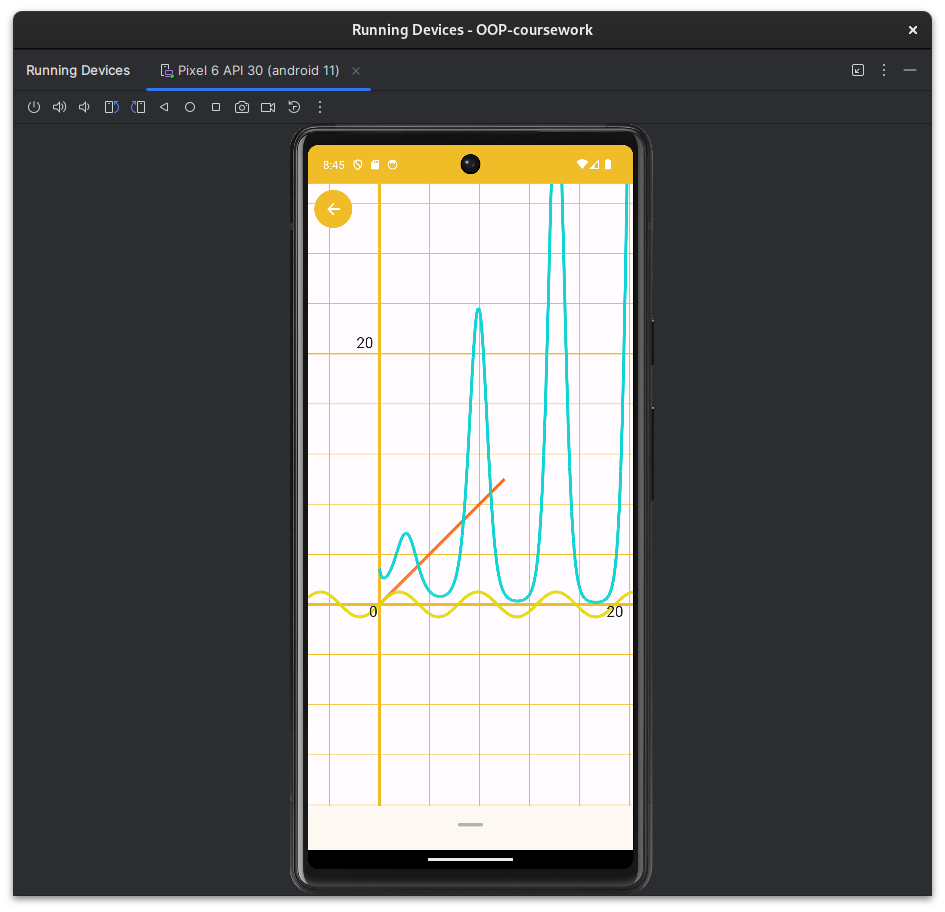
\includegraphics[width=\textwidth]{1}
% 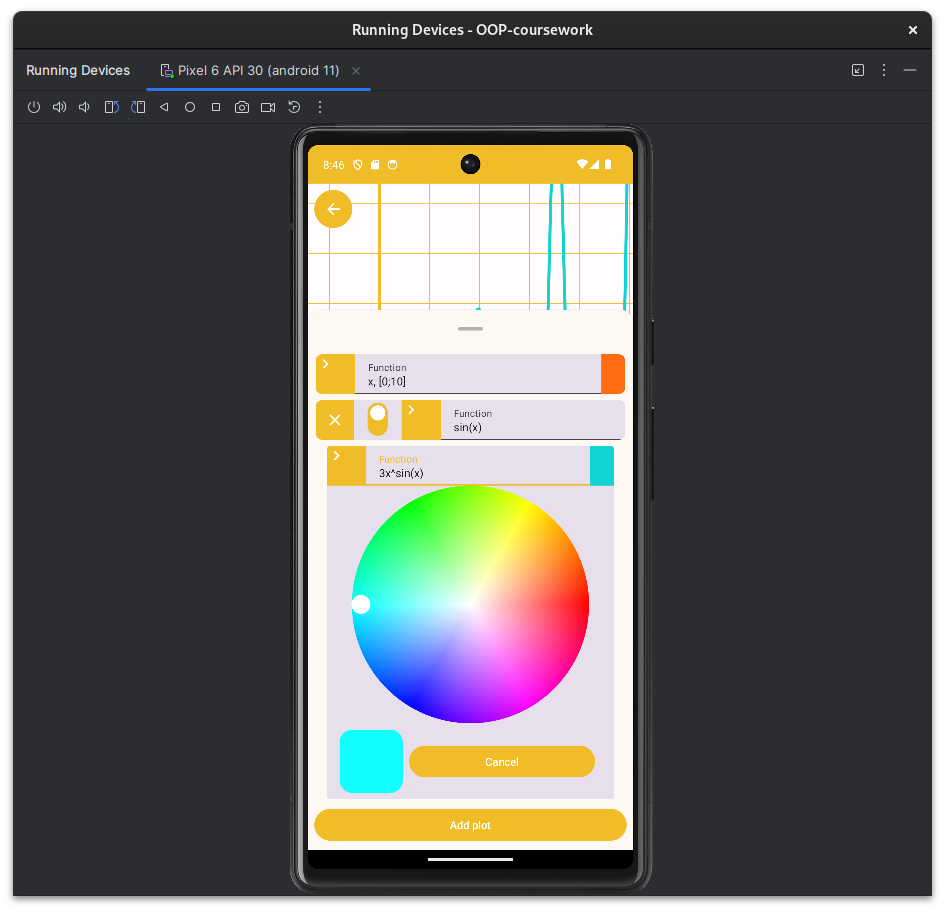
\includegraphics[width=8cm]{2}
\centering
\end{figure}


% include pdf
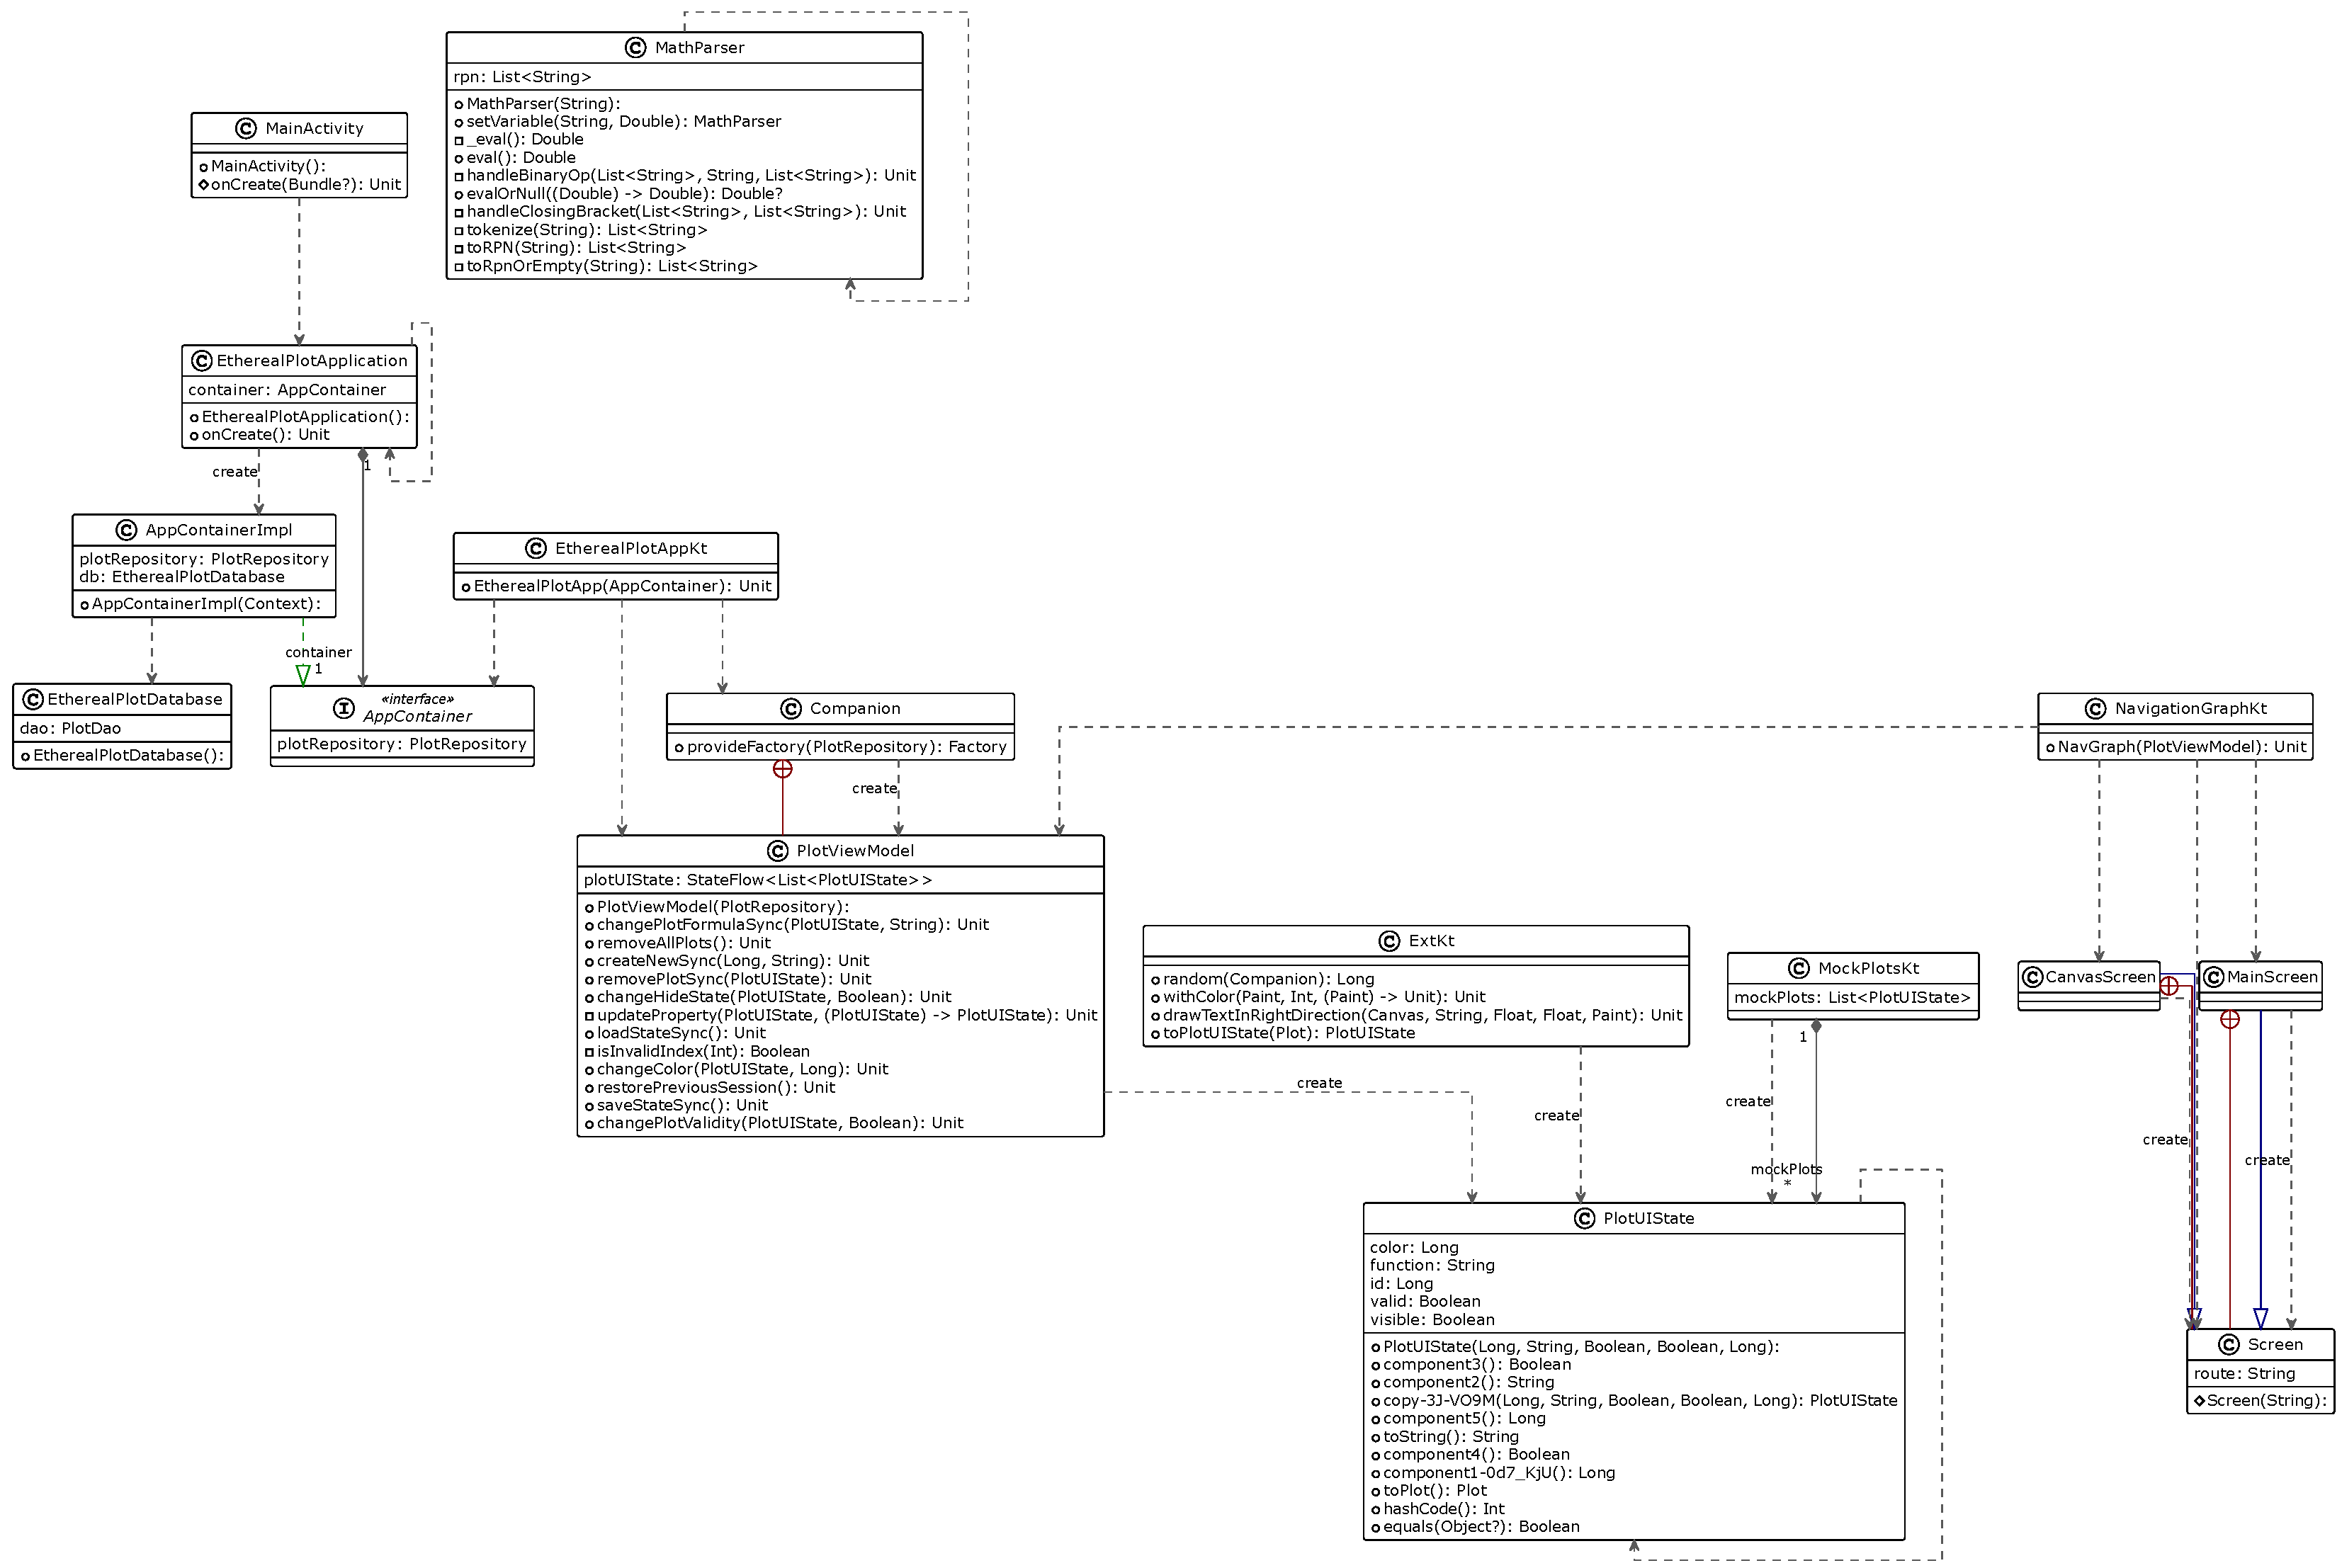
\includepdf[pages=-]{pictures/package.pdf}



    \section{Висновки:}
У даній теоретичній частині було розглянуто ключові аспекти, пов'язані з розробкою програми для побудови графіків довільних функцій на платформі Android з використанням Jetpack Compose. Основні висновки можна сформулювати наступним чином:

\begin{enumerate}
    \item \textbf{Графічні Двигуни та Бібліотеки:} Було проведено аналіз різних графічних двигунів та бібліотек для побудови графіків, і Jetpack Compose виявився потужним та сучасним інструментом з багатим функціоналом.

    \item \textbf{Jetpack Compose та Kotlin:} Вибір Jetpack Compose та мови програмування Kotlin був обґрунтований їх сучасністю, продуктивністю та підтримкою Android. Це сприяє ефективній розробці та забезпечує чистий та читабельний код.

    \item \textbf{Реактивне Програмування:} Використання концепцій реактивного програмування дозволяє ефективно взаємодіяти з графічним інтерфейсом, роблячи його більш відзивчивим та динамічним.

    \item \textbf{Архітектурні Підходи:} Використання архітектурного підходу MVVM дозволяє ефективно розділити логіку програми та відображення, полегшуючи підтримку та розширення.

    \item \textbf{Тестування в Android:} Стратегії тестування, такі як юніт-тестування та інтеграційне тестування, є необхідним елементом для забезпечення стабільності та надійності програми.

\end{enumerate}

В цілому, теоретичний аналіз дозволяє визначити оптимальний напрям для подальшого розвитку проекту "Ethereal Plot" та забезпечує підґрунтя для успішної реалізації практичної частини. 

\end{document}
